\begin{figure}[h]
    \centering
    
\includegraphics[width=0.3\textwidth]{chocolate-chip-cookies-author}
    \caption{Luciano van der Toorn, Athens, Greece}
\end{figure}

\noindent\textbf{Bio:}\\
Luciano has been a passionate hobby baker for years
and then decided to focus his efforts on launching
a micro bakery in Greece. He is passionate about
fermenting and making people happy with great bread.

\noindent\textbf{About this recipe:}\\
Dive into a world of decadence with these chocolate chip cookies,
where every bite boasts the perfect balance of crisp edges and a soft,
chewy center. Studded generously with melt-in-your-mouth chocolate chunks,
each cookie promises a burst of rich flavor that'll leave you craving just one more.
Handcrafted with love and baked to golden perfection,
these cookies are the ultimate treat for both casual snackers and discerning dessert aficionados.

\begin{figure}[h]
    \centering
    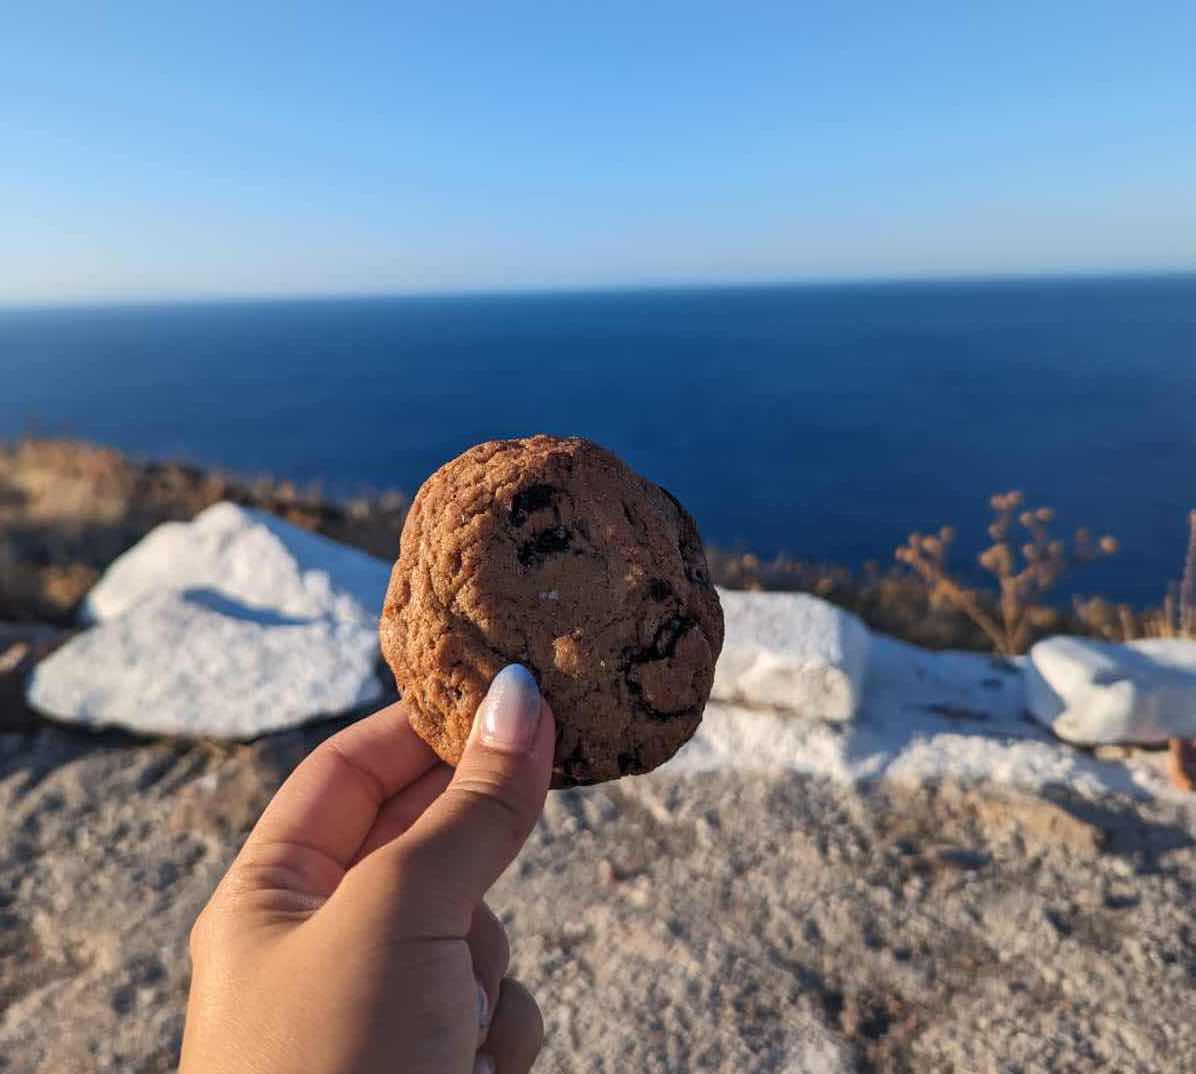
\includegraphics[width=0.6\textwidth]{chocolate-chip-cookies.jpg}
    \caption{The chocolate chip cookies this recipe makes}
\end{figure}

\noindent\textbf{Ingredients:}

\begin{center}
\begin{tabular}{|c|l|r|}
    \hline
    \textbf{No.} & \textbf{Ingredient} & \textbf{Quantity} \\
    \hline
    1 & Butter, cubed & 115 g \\
    \hline
    2 & Butter, cubed & 55 g \\
    \hline
    3 & Dark brown sugar & 210 g \\
    \hline
    4 & White sugar & 50 g\\
    \hline
    5 & Egg & 1 pc \\
    \hline
    6 & Egg yolk & 2 pcs \\
    \hline
    7 & Vanilla extract & 2 tsp \\
    \hline
    8 & Bread flour & 210 g \\
    \hline
    9 & Salt & 4 g \\
    \hline
    10 & Baking soda  & 4 g \\
    \hline
    11 & Choc. chips, 60-70\% cocoa & 170 g\\
    \hline
\end{tabular}
\end{center}

\noindent\textbf{Instructions:}
\begin{center}
\begin{tabular}{|c|p{12cm}|}
    \hline
    \textbf{Step} & \textbf{Instruction} \\
    \hline
    1 & On medium heat, brown the \#1 until dark brown. Add to mixing bowl and let cool for 1 minute. \\
    \hline
    2 & Add \#2 to the mixing bowl (should not sizzle/foam), wait until everything is melted. \\
    \hline
    3 & Add \#3 and whisk until no clumps remain, ±30s. Add \#5, mix until incorporated. \\
    \hline
    4 & In a separate bowl, add all ingredients from \#6 and mix briefly. \\
    \hline
    5 & Add mix from step 3 to the mix of step 4, fold using rubber spatula until no dry spots remain. \\
    \hline
    6 & Fold \#7 into mixture. Do not over-mix to prevent gluten formation. \\
    \hline
    7 & Refrigerate (2-5°C) for at least 6 hours, max 5 days, or freeze max 6 months. \\
    \hline
    8 & Using ice cream scoops (size 24/20/16), make round balls and place on parchment lined sheets. \\
    \hline
\end{tabular}
\end{center}

\noindent\textbf{Baking:}
\begin{center}
\begin{tabular}{|c|p{12cm}|}
    \hline
    \textbf{Step} & \textbf{Instruction} \\
    \hline
    1 & Baking in pre-heated oven set to 200C. Just before baking, using ice cream scoop (size 24, 20, or 16): Make round balls and place on parchment lined baking sheets. 60x40cm baking sheet holds 6 or 8 cookies. \\
    \hline
    2 & Bake for 10-14 min. at 200°C, no steam. \\
    \hline
    3 & For size 20 scoop: Bake for 14 minutes in deck oven. \\
    \hline
    4 & For size 24 scoop: Bake for 13 minutes in deck oven. \\
    \hline
\end{tabular}
\end{center}
